\section{Literature review}

My research is located at the intersection of three main subjects:
\begin{itemize}
	\item Interactive music systems for non-professional musicians,
	\item modern, technology dependent, social phenomena
	\item and social effects of music.
\end{itemize}
I will start this review with a brief introduction to the field of interactive music systems, followed by a short description of each of the above subjects, elucidating only the aspects relevant to my research.
This review will end with a research road map which will present how those different fields combines together and their importance to this work.
Lastly, the system will be described, as a whole, from the participant point of view.

\subsection{A brief introduction to interactive music systems}

According to the Oxford Dictionary to ``interact'' is to ``act in such a way as to have an effect on each other'' (\cite{web:oxford}).
``Act'' and ``affect'' are visibly the main concepts of interactivity.
In the field of interactive music systems these ideas may be implemented in different ways, ranging from new instrument designs to collaborations with robotic performers (\cite{drummond09}).

Since the beginning of the exploration in the field of interactive music systems in the nineteen-sixties, different researchers and composers created systems that were designed to interact with performer in a live situation.
First example of this kind of interactive system was Gordon Mumma's Hornpipe, where specially designed electronic system alters the sound of the audio input from the performer and creates an interactive loop between the player and the resultant sound of the electronics circuit (\cite[page 12]{winkler01}).

In the same tame, and continuously during the nineteen-seventies, programming languages designed for musical applications, such as GROOVE or the MUSIC-N series, began to be developed (\cite{mathews70}; \cite{mathews69}).
Using those languages musicians and researchers was able to create interactive music systems programmatically, as opposed to electronically designed systems like those of Mumma.

In the nineteen-eighties, a group of musical instruments manufacturers agreed on standard method for sending and receiving musical information digitally, establishing the MIDI protocol as a universal standard (\cite{web:quinn}).
The standardization of sending and receiving information combined with the emergence of personal computers enabled the creation of modern programing languages for musical applications.
Max/MSP, which began its development by Miller Puckette in 1986, may be a good example (\cite[page 16]{winkler01}).
As opposed to early programming languages as GROOVE or the MUSIC-N series, most of those personal computer based languages still exist today, keep progressing and new music oriented programing languages are developed on a regular basis (\cite{web:chuck}; \cite{web:usine}).

In addition to the development of modern programming languages for music applications the proliferation of the personal computer also opened new possibilities for live performance.
During the nineteen-nineties digital audio workstations (DAW) became a common alternative to analog recording equipment in studios (\todo{find ref}).
Later, with the arrival of the VST standard (\cite{web:steinberg}), computers became even more essential tool for music production.
The arrival of those technologies to the stage could be identified with the emergence of live performance oriented DAWs as Ableton Live (\cite{web:live}) and software based DJ setups in late nineteen-nineties.

Another key event in the history of interactive music systems is the appearance of the Arduino platform in 2006.
The Arduino is an easy to use hardware and software package, ``intended for artists, designers, hobbyists and anyone interested in creating interactive objects or environments'' (\cite{web:arduino}).
Until its appearance the only way for a musician to interact with music creation software was through audio and MIDI.
But from then a lot of new ways of controlling audio started to be possible, mostly by translating physical properties of the space into sound.

\subsection{Interactive music systems for non-professional musicians}

In addition to systems that interact with a performer or professional musician there are also interactive music systems for non-professional musicians.
In the following paragraphs I will show some different approaches to this concept.

% interactive video clips: Interlude, Chris Milk and Aaron Koblin
Recently, a new type of interactive video clips started to emerge.
Those video clips expose some of the roles traditionally kept for the director, to the viewers.
As a relatively new phenomena video clips like those are rare but prominent.
As examples one can find the works of Chris Milk and Aaron Koblin (\cite{web:milk1}; \cite{web:milk2}) and the startup Interlude which driven by equivalent concept (\cite{web:interlude}).

% mobile applications: Smule and RjDj
The emergence of modern mobile phones with their high computation power led developers to develop new mobile applications for music creation for non-professional musicians.
Those applications gives the average user the ability to create music by himself and without musical education.
Good examples for this kind of applications are Smule's applications, with emphasis on AutoRap (\cite{web:autorap}).
On the other hand, the same technology open the opportunity to consume interactive music or rather ambient sonification that affected by the user surrounding as demonstrated by RjDj (\cite{web:rjdj}).

% interactive sound installations: objects with sound, project ADA
Sound installations are installations located in the three dimensional space that dialog with their surroundings through sound (``\citetitle{wiki:soundinstallation}'').
Whereas in some interactive sound installations the main interaction is between the viewer and the installation itself (\cite{web:visnjic}) there are installations that aims to engage the participants to interact with one another (\cite{eng03}).
One may say that the main goal of this kind of interaction is to facilitate social interaction\todo{find ref, maybe Omer Golan}.

% social DJing: DistributedDJ, the BLOB and playmysong
Furthermore, recent projects suggest a framework to share the role of the DJ in a bar or party between the participants (\cite{web:shaw}).
Using those systems participants can choose the music by themselves and the ``playlist'' is created dynamically by their musical taste of the participants.
Most of those project are implemented as mobile applications and some them even integrate social elements in their projects (\cite{web:playmysong}; \cite{web:lammers}).

% summarize the interactivity trend
Although the above researches and projects are only a small portion of the work that has been done in the field of interactive music systems for non-professional musicians it clearly demonstrates how new technology could be used to allow the average user to participate both in interactive music creation and consumption, as well as in the social interactions those processes present.

\subsection{Modern, technology dependent, social phenomena}

% Silent disco and flash mobs. LBS are out because they are not really relevant!

The fast growth of social media produced modern types of social behavior.
Two particular phenomena that emerged from this situation that are relevant to my study are silent disco, and flash mobs.

Silent disco is the phenomenon of partying where the music is heard through headphones instead of loudspeakers.
The origins of the phenomena are unclear, but it began to be an ordinary way of partying toward the beginning of 2000's (``\citetitle{wiki:silentdisco}'').
The new phenomena already changed the possibilities of an ordinary party.
One new possibility was having two DJs spin two completely different sets side by side at the same party where each participant has two channel wireless headphones, and can decide which DJ to listen to (\cite{web:headphonedisco}).
Needless to say, this is not possible with a regular loudspeaker setup.

Another phenomenon relevant to my research is that of flash mobs: ``A group of people who assemble suddenly in a public place, perform an unusual and seemingly pointless act for a brief time, then quickly disperse, often for the purposes of entertainment, satire, and artistic expression. Flash mobs are organized via telecommunications, social media, or viral emails'' (``\citetitle{wiki:flashmob}'').
With regards to the definition above, with emphasis on the way flash mobs are organized and executed, different researchers see the flash mobs as a significant event in the history of mobile communication (\cite{nicholson05}).
On the other hand, a recent study by Brejzek suggests that a potential for artistic intent inherently exists in the flash mob phenomenon (\cite*{brejzek10}).

\subsection{Social effects of music}

% Based, as suggested by Avi, on ``The social psychology of music -- David Hargreaves''.

\subsection{Roadmap}\label{roadmap}

% Describe the system and its connection with concepts mentioned before. Everything bellow is new!

The system developed in this research is inspired by the concepts of interactive music systems and intended for the average user.
It sees both silent disco and flash mobs as significant conceptional roots.
Whereas silent disco will be referred as a context for the system existent, flash mobs are associated as a social phenomena that use new technologies to facilitate creative, or even artistic social behavior, with emphasis on social interaction.

From the participants point of view the system will consist of few balloon bundles, each one corresponds to a specific musical style.
When the participants will stroll between the balloon bundles with their mobile devices and headphones their relative distances from the different bundles will affect the music in their headphones, creating virtual ``sound zones'' around each balloon bundle.
The distance between each participant and sound zones may affect the music in several different ways.
For example, when a participant get close to specific sound zone the music filtration may change according to the distance.
For another sound zone the volume may be changed when getting close to it or walk away.
Although the style of each sound zone will be well-definition, every sound zone will by able to be heard with any other sound zone, in synchronization and harmony.
In addition, participants will be able to freely move the balloon bundles, thereby changing the structure of the music in the virtual space\footnote{A video demonstrating the system behavior from the participant point of view can be found at \href{http://youtu.be/2kJoeD2iWBA}{youtu.be/2kJoeD2iWBA}.}.

\begin{figure}[h]
	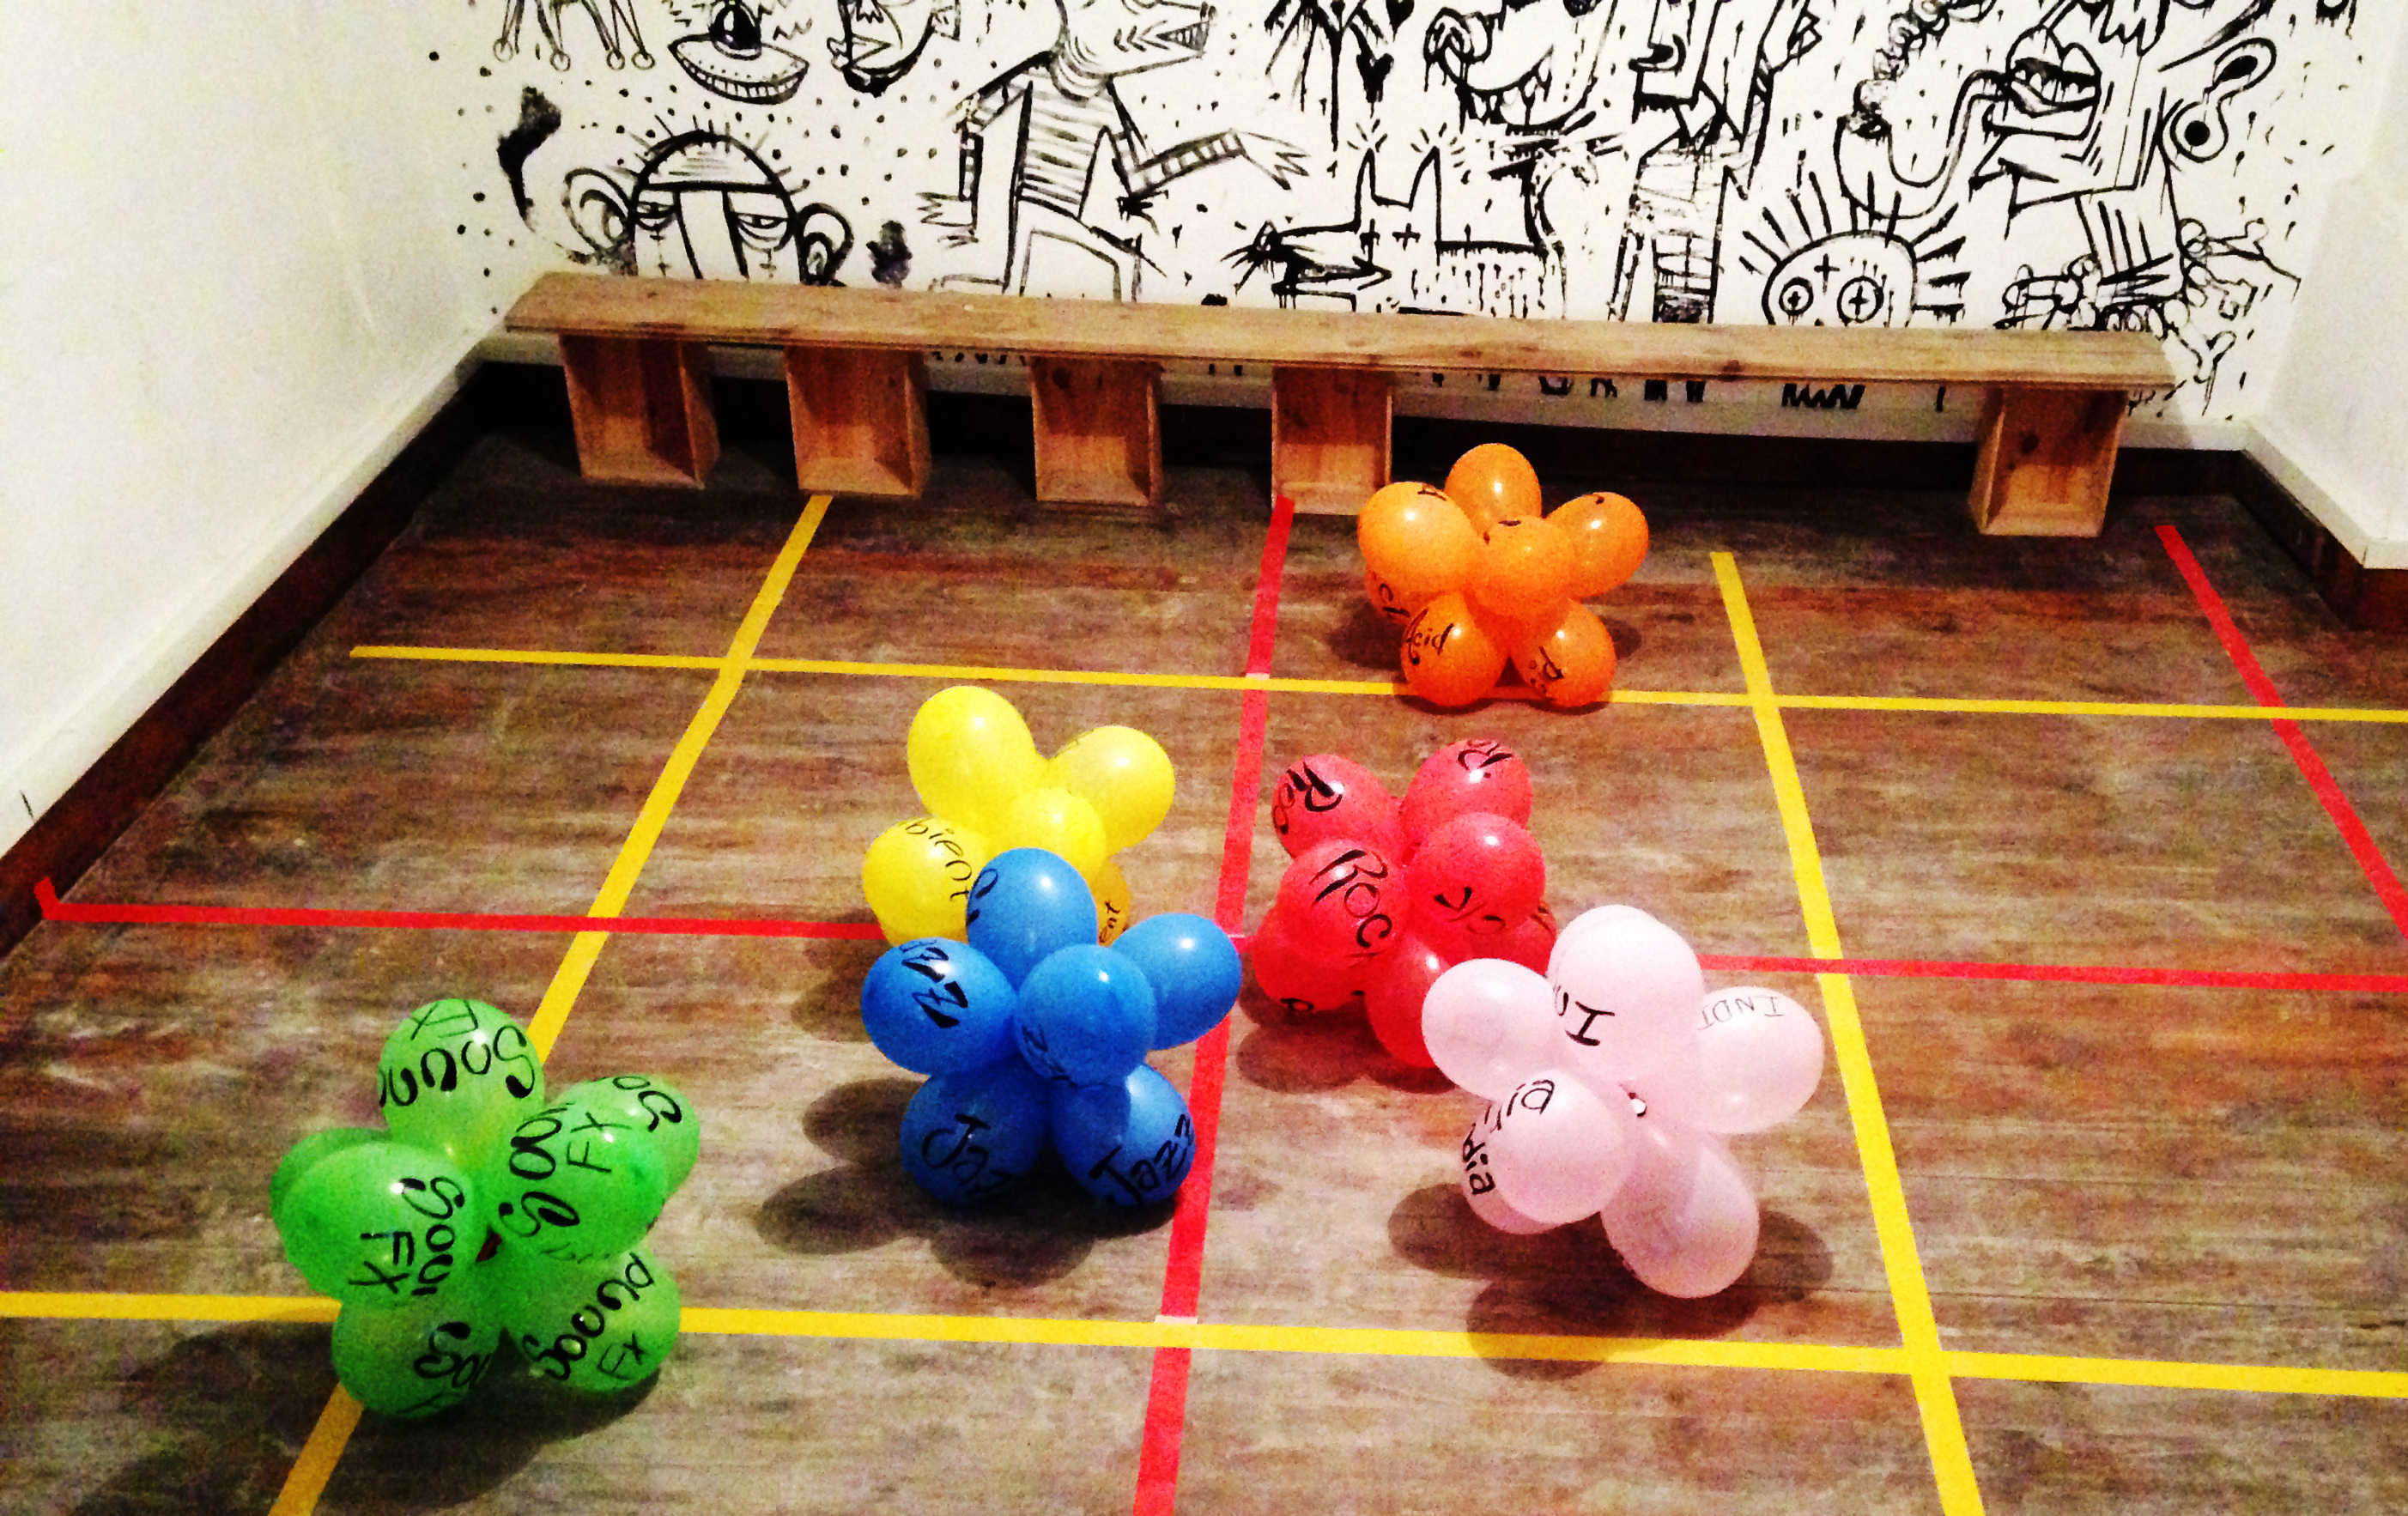
\includegraphics[width=\linewidth]{balloons}
	\caption{Balloon bundles on the dance floor}
\end{figure}

In order to evaluate the social effect of this system I will try to answer the research question: \emph{\reserchquestion}